\chapter{Pendolo su carrello}
\section{Modello del motore}
\begin{center}
	\includegraphics[width=\textwidth]{motoreSimulink.jpg}
\end{center}
Il LEGO MINDSTORM EV3 è dotato di un motore, l'EV3 Large Servo Motor, la cui velocità, misurata in $rad/s$, è stata assunta come uscita del sistema.\\
I valori di ingresso possibili sono invece compresi tra -100 e +100, dove +100 indica la massima potenza, mentre -100 idem, ma con verso di rotazione opposto.\\
Al fine di modellare nel modo più preciso possibile abbiamo applicato a tale motore un albero dotato di pesi posti a una certa distanza da quest'ultimo in modo tale da incrementare il momento d'inerzia $I$ e, di conseguenza, diminuire l'accelerazione angolare massima $\alpha$ in accordo con la seconda legge di Newton in forma angolare $\tau = I\alpha$ dove $\tau$ indica il momento della forza o, più semplicemente, la coppia massima erogata: valore caratteristico del motore.
\begin{center}
	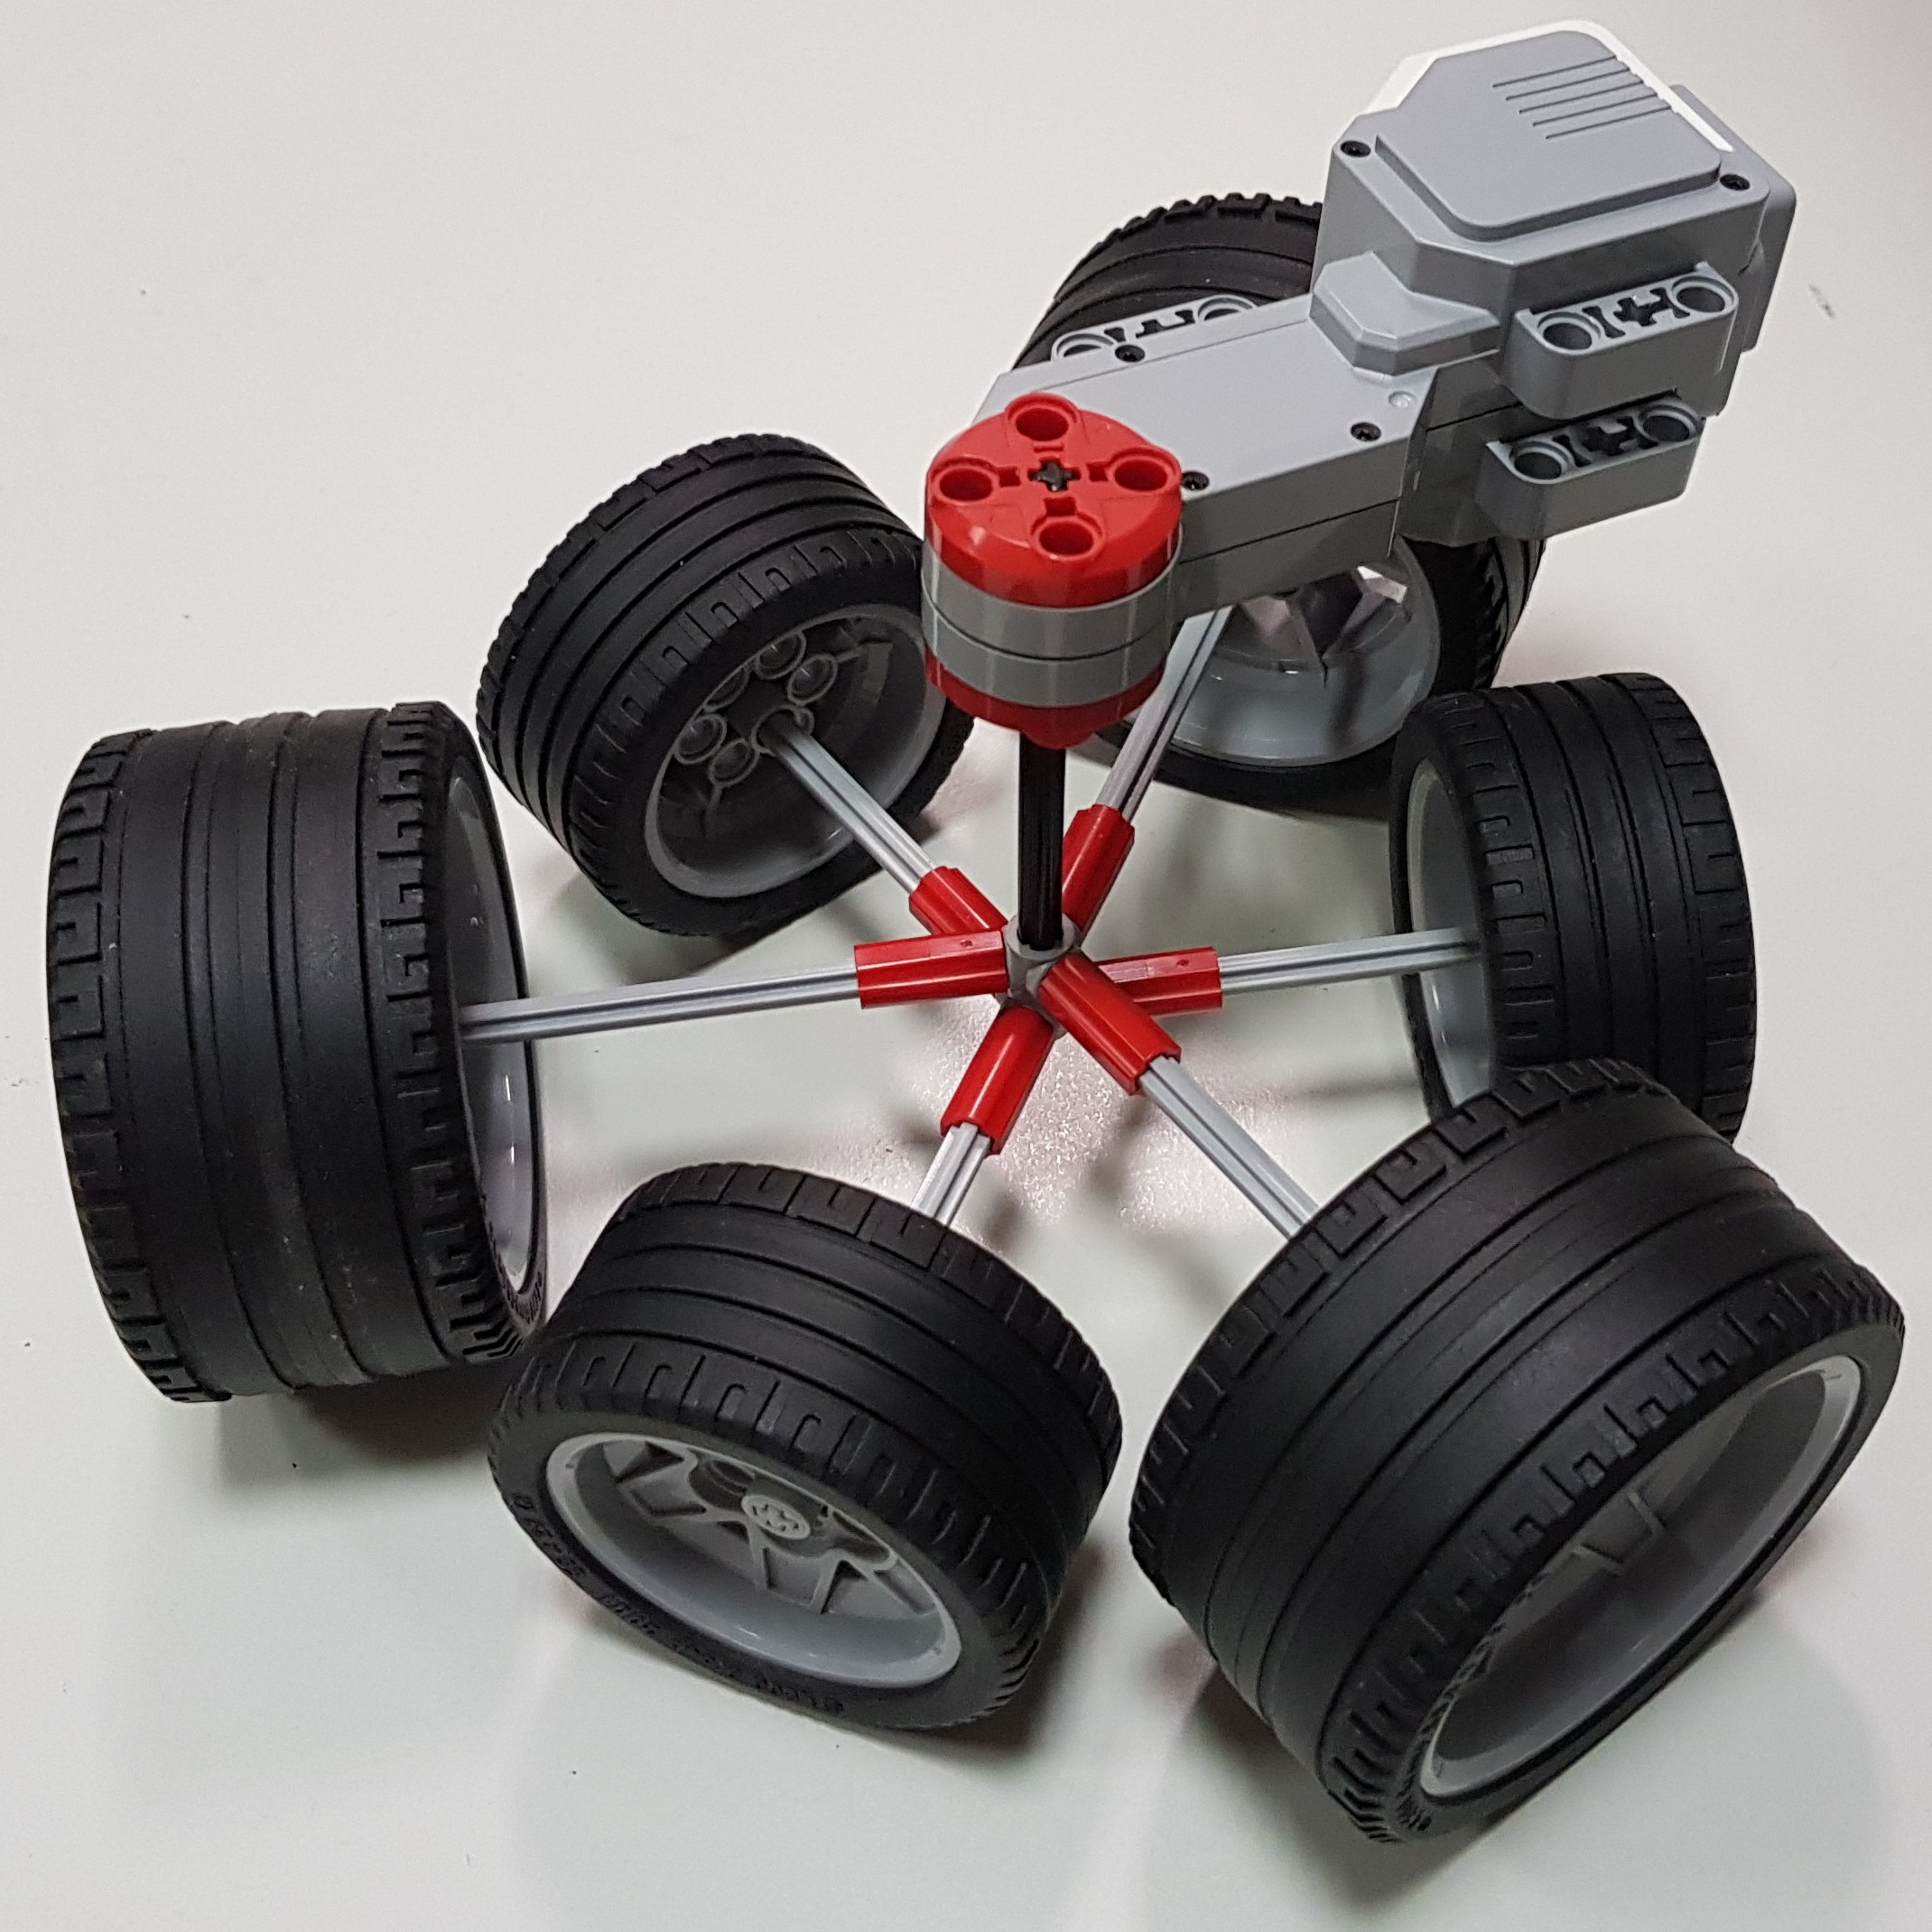
\includegraphics[width=\textwidth]{megainerzia.png}
\end{center}
In questo modo il tempo di assestamento $t_a$ del sistema, direttamente proporzionale a $\alpha$, è sensibilmente più lungo ed è dunque più semplice trovare una funzione di trasferimento assimilabile a quella dell'EV3 Large Servo Motor.\\
L'encoder presente all'interno del motore è poi in grado di misurare, in $rad$, la rotazione dello stesso.
Di conseguenza, al fine di ottenere la velocità angolare $\omega$ è stato applicato in cascata un derivatore, ma anche un filtro low-pass con frequenza di taglio $\omega_c=25\;Hz$, necessario per attenuare le alte frequenze del sistema al fine di ottenere una funzione di trasferimento meno spezzata possibile.\\
Per l'encoder è stato invece scelto un tempo di campionamento di 0.001 $s$, il minimo supportato.\\
Il risultato che si ottiene utilizzando come ingresso una funzione gradino con valore finale pari a 50 è mostrato nella figura seguente:
\begin{center}
	\includegraphics[width=\textwidth]{motore50StepCamp1000.jpg}
\end{center}
Scegliendo invece una frequenza di taglio del LPF $\omega_c = 100Hz$ la funzione di trasferimento diventa:
\begin{center}
	\includegraphics[width=\textwidth]{motore50StepCamp1000Polo100.jpg}
\end{center}
Si può notare come la frequenza di taglio sia troppo alta rendendo così impossibile la stima della funzione di trasferimento.\\
Prendendo quindi in esame il primo dei due grafici si può stimare una costante di tempo $\tau$ del sistema pari a circa 0.15 $s$ e guadagno 10.4.\\
La funzione di trasferimento che ne consegue è dunque:
\\
$$
T_m(s)=\displaystyle\frac{10.4}{0.15s+1}
$$
\\\\
Di seguito un confronto tra $T_m(s)$ e la funzione di trasferimento reale del motore.
\begin{center}
	\includegraphics[width=\textwidth]{modMotorvsReale.jpg}
\end{center}
\section{Dalla velocità angolare alla coppia}
A questo punto è necessario ottenere la coppia generata dal motore in funzione del tempo al fine di utilizzarla come ingresso per la funzione di trasferimento del pendolo che sarà trattata nel prossimo capitolo.\\
La formula utilizzata per calcolare tale coppia è la seguente:
$$
\tau=K\omega+I\alpha
$$
Dove $\tau$ indica appunto la coppia, $K$ il coefficiente di smorzamento viscoso misurato in $Nm\,s/rad$, $\omega$ la velocità angolare, $I$ il momento d'inerzia del sistema e $\alpha$ l'accelerazione angolare.\\
Calcoliamo innanzi tutto $I$: 
$$
I=3Ml^2+3ml^2+6I_{asta}
$$
Il primo coefficiente indica il momento d'inerzia generato dalle tre ruote grandi, il secondo da quelle piccole, mentre il terzo dalle sei aste che collegano le ruote all'albero, di lunghezza $l$.\\
Per calcolarlo utilizziamo il teorema di Huygens-Steiner, o degli assi paralleli:
$$
I=I_{cdm}+m_{asta}d^2
$$
Dove $d$ è la distanza dell'asta dal centro di massa.\\
Si ottiene dunque:
$$
I_{asta}=\displaystyle\frac{1}{12}m_{asta}l^2+m_{asta}(\displaystyle\frac{l}{2})^2=\displaystyle\frac{1}{3}m_{asta}l^2
$$
Sostituendo i valori di masse e lunghezze misurati si ricava un momento d'inerzia $I$ pari a 0.001364 $Kg\,m^2$.\\
Essendo $\tau=K\omega+I\alpha$ possiamo disegnare con Simulink il seguente diagramma a blocchi:
\begin{center}
	\includegraphics[width=\textwidth]{modMotoreTorque.jpg}
\end{center}
L'uscita del sistema è proprio la coppia $\tau$ desiderata.\\
Si può notare come nel blocco inferiore siano stati aggiunti il derivatore e il LPF di cui è stato discusso precedentemente.\\
Il primo è necessario dal momento che per ottenere l'accelerazione angolare $\alpha$ bisogna derivare la velocità angolare $\omega$.\\
Per quanto riguarda il LPF, invece, è stato aggiunto dal momento che un derivatore puro è fisicamente irrealizzabile (funzione strettamente propria).\\
Il valore di K è stato invece scelto pari a 0.0006 $Nm\,s/rad$ come da specifiche dell'EV3 Large Servo Motor.\\